\section{Barycentric coordinates}
Let us consider a triangle with top, bottom left and bottom right vertices to which we have assigned the colors red, green and blue respectively. The triangle barycentre divides each median into two parts that have a 2:1 ratio. \\
  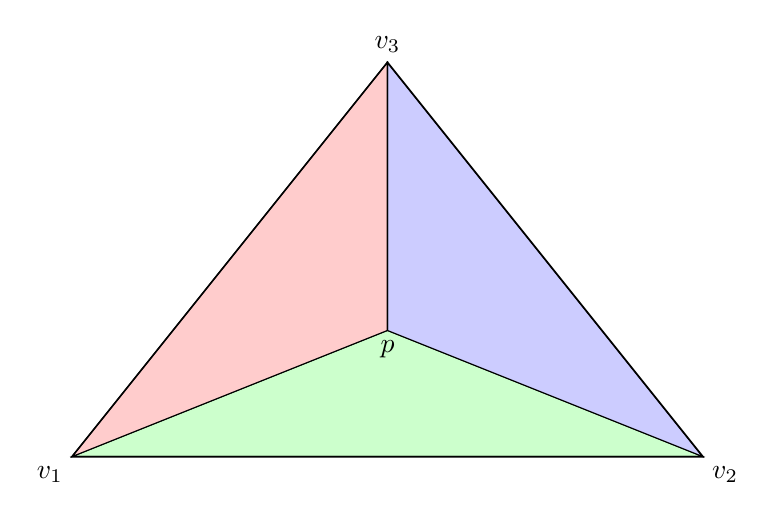
\begin{tikzpicture}
    \coordinate (L1) at (0,0);
    \coordinate (L2) at (8,0);
    \coordinate (L3) at (4,5);
    \coordinate (X) at (4,1.6);

    \draw[thick] (L1) -- coordinate[midway](md3) (L2)
                      -- coordinate[midway](md1) (L3)
                      -- coordinate[midway](md2) (L1) -- cycle;
    \filldraw[draw=black, fill=green!20] (L1) -- (X) -- (L2) -- cycle;
    \filldraw[draw=black, fill=red!20] (L1) -- (X) -- (L3) -- cycle;
    \filldraw[draw=black, fill=blue!20] (L3) -- (X) -- (L2) -- cycle;
    \draw (L1) node [below left] {$v_1$}
       -- (L2) node [below right] {$v_2$}
       -- (L3) node [above] {$v_3$}
       -- (X) node [below] {$p$};
    \end{tikzpicture}
    \\
    Let call the red area $w_1$, the blue green one $w_2$ and the blue one $w_3$. Normalazing each of them by the area of the triangle, we will get three values ($\lambda_1, \lambda_2, \lambda_3$) that are the barycentric coordinates of $p$ with respect to the triangle [$v_1, v_2, v_3$].
\\ \\ WRITE introduction of Barycentric coordinate (inventor and history) and all properties

\section{Triangle mesh}
See book


\section{Lighting}
formula + draw and explanation of angle (like at 90 degree some light..e.tc.)

\section{Linear Interpolation}
The standard linear interpolated visualisation is made passing three attributes (colors) for each vertex of a triangle. OpenGL will interpolate linearly the colors. That is possible thanks to the barycentric coordinates that will tell how much of each color is being mixed at any position.

\section{Flat Shading}

\section{Gouraud Shading}
\textit{Gouraud Shading} can be calculated in the \textit{vertex shader}. The main idea is to compute a normal at the vertex and an intensity for each vertex.

\section{Curvature}
\subsection{Gaussian Curvature}
\textit{Gaussian Curvature} works like a logical \texttt{AND}, it will check if there is a curvature along both directions.

\begin{figure}[h]
  \minipage[b]{.6\linewidth}
  \centering
  \scalebox{0.7}{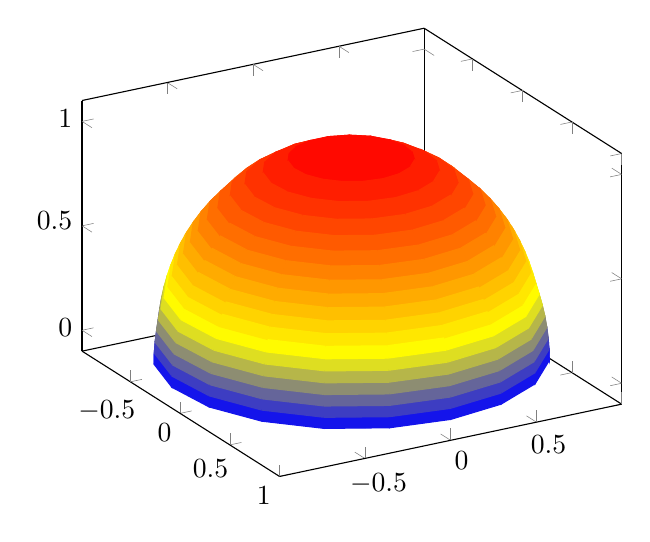
\begin{tikzpicture}
  \begin{axis}[view={60}{30}]
      \addplot3[surf,shader=flat,
          samples=20,
          domain=1:0,y domain=0:2*pi,
          z buffer=sort]
          ({sqrt(1-x^2) * cos(deg(y))},
       {sqrt( 1-x^2 ) * sin(deg(y))},
       x);
  \end{axis}
  \end{tikzpicture}}
  \caption{Positive gaussian curvature}\label{fig:positive-gaussian}
  \endminipage
  \minipage[b]{.6\linewidth}
  \centering
  \begin{tikzpicture}[scale=0.7]
    \begin{axis}[view={60}{30}]
    \addplot3[patch,patch refines=3,
    shader=faceted interp,
    patch type=biquadratic]
    table[z expr=x^2-y^2]
    {
        x  y
        -2 -2
        2  -2
        2  2
        -2 2
        0  -2
        2  0
        0  2
        -2 0
        0  0
    };
  \end{axis}
  \end{tikzpicture}
  \caption{Negative gaussian curvature}\label{fig:negative-gaussian}
  \endminipage
\end{figure}
Surfaces that have a zero gaussian curvature are called \textit{developable surfaces} because they can be flattened out into the plane without any stretching. Gaussian curvature should be zero inside each mesh triangle and the same along edges since it can be flattened symmetrically into the plane.

\subsection{Mean Curvature}


